 % !TEX TS-program = pdflatex
% !TEX encoding = UTF-8 Unicode



\documentclass[10pt]{article}

\usepackage[francais]{babel}
\usepackage[T1]{fontenc}
\usepackage[utf8]{inputenc}

\usepackage{amsmath,amsfonts,amssymb,ulem,epigraph}

\usepackage[upright]{fourier}

\usepackage{shadethm}

\usepackage{subfig}

\usepackage{pgf,tikz}
\usetikzlibrary{arrows}

\usepackage{color}
\definecolor{gris_clair}{gray}{.9}
\definecolor{gris}{gray}{.35}
\definecolor{vert}{rgb}{0,0.5,0}
\definecolor{rouge}{rgb}{0.5,0,0}
\definecolor{turquoise}{rgb}{0,0.5,0.5}

\usepackage{listings}           
\lstset{
language=Caml,
backgroundcolor=\color{gris_clair},
frame=single,
basicstyle=\footnotesize\ttfamily\color{gris},
identifierstyle=\color{black},
keywordstyle=\color{vert},
stringstyle=\color{rouge}, showstringspaces=false,
commentstyle=\itshape\color{turquoise},
%numbers=left, numbersep=5pt, numberstyle=\color{gris}\tiny,stepnumber=5,
breaklines=true,
literate=
  {é}{{\'e}}1 {É}{{\'E}}1 {à}{{\`a}}1 {è}{{\`e}}1% 
  {À}{{\`A}}1 {È}{{\'E}}1 {ë}{{\"e}}1 {ï}{{\"i}}1%
  {â}{{\^a}}1 {ê}{{\^e}}1 {î}{{\^i}}1 {ô}{{\^o}}1% 
  {û}{{\^u}}1 {Â}{{\^A}}1 {Ê}{{\^E}}1 {Î}{{\^I}}1%
  {Ô}{{\^O}}1 {œ}{{\oe}}1 {Œ}{{\OE}}1 {æ}{{\ae}}1%
  {Æ}{{\AE}}1 {ç}{{\c c}}1 {Ç}{{\c C}}1 {€}{{\EUR}}1%
  }

\graphicspath{{./} {./../presentation-tipe/}}

\title{Autour du Manège Enchanté}
%\subtitle{intersections routières}
\date{}
\author{Antonin Dudermel}

\begin{document}

\newshadetheorem{defin}{Définition}
\newshadetheorem{theo}{Théorème}

\maketitle

\section{Un Graphe pour le Manège}
	\subsection{Le Manège}
	
Le Manège enchanté est un rond-point assez particulier situé sur une intersection à 5 voies à Swindon en Angleterre : il est composé de 5 petits ronds-points tournant dans le sens anti-horaire (comme les ronds-points anglais) disposés en périphérie d'un grand rond-point central tournant dans le sens inverse, la priorité étant aux voitures situés à l'intérieur des petits ronds-points, comme le montre la figure \ref{rp}.
\begin{figure}
	\begin{center}
		\caption{\label{rp}le manège enchanté}
		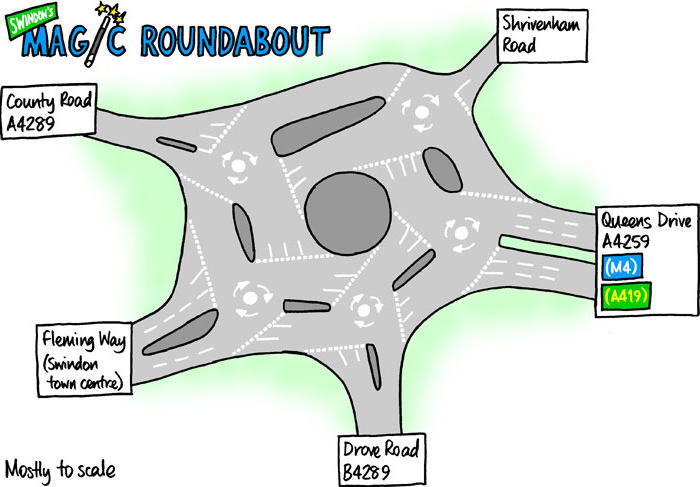
\includegraphics[scale=0.4]{images/magic-brit}
	\end{center}
\end{figure}

Une telle disposition permet une diversité des itinéraires possibles pour aller d'une entrée à une sortie (voir figure \ref{itin}). Le manège serait grâce à cela une réponse plus efficace au problème des intersections routières : assurer un trafic le plus fluide possible, des distances plus courtes, des infrastructures plus sûres… L'objectif de ce TIPE est de montrer que le manège enchanté remplit bien de telles conditions. Nous avons pour cela mis en place deux modèles : un utilisé en pratique pour étudier des infrastructures routières, par automates cellulaire, mais face à la complexité de ce modèle, nous nous sommes rabattus sur une étude plus élémentaire {\it via} la théorie des graphes.

\begin{figure}
		\begin{center}
			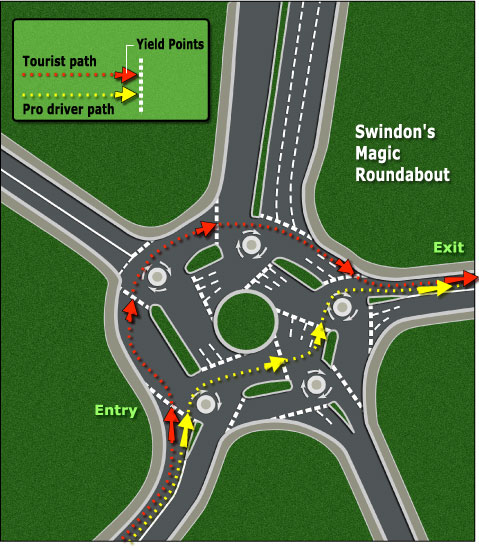
\includegraphics[scale=0.3]{images/itin}
			\caption{\label{itin} itinéraires possibles}
		\end{center}
	\end{figure}


	\subsection{Modéliser par un graphe}

On peut aisément représenter un ensemble de routes par un graphe orienté pondéré : il suffit de considérer chaque intersection comme un sommet et chaque route comme une arête reliant une intersection à une autre de poids la longueur de la route. En appliquant ce principe au manège enchanté, on aboutit au graphe représenté par la figure \ref{grman}. De même on peut construire un graphe représentant le rond-point formé par la périphérie du manège. \par
L'intérêt principal de l'étude étant plus la forme du manège que cet exemple particulier, par souci d'implantation, le graphe a encore été simplifié en considérant les sorties et les intersections internes disposées en pentagones réguliers.

\begin{figure}
		\begin{center}
			\subfloat[le manège]{%
				\label{grman}
				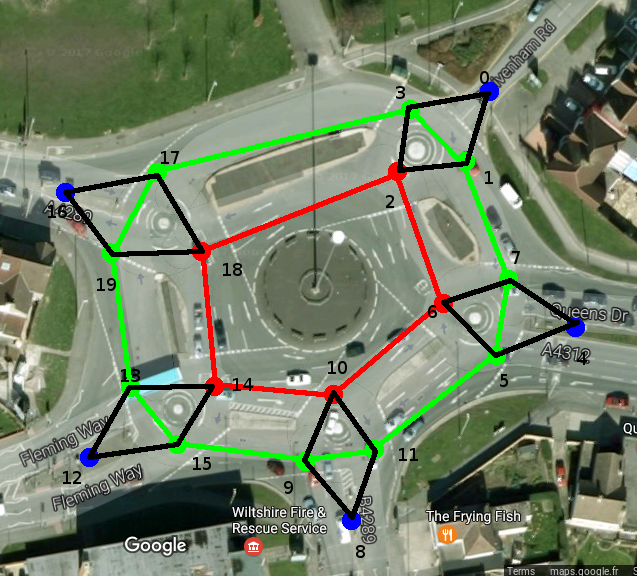
\includegraphics[scale=0.2]{../manege-graphe}
				}
			\subfloat[le rond-point]{%
				\label{grrp}
				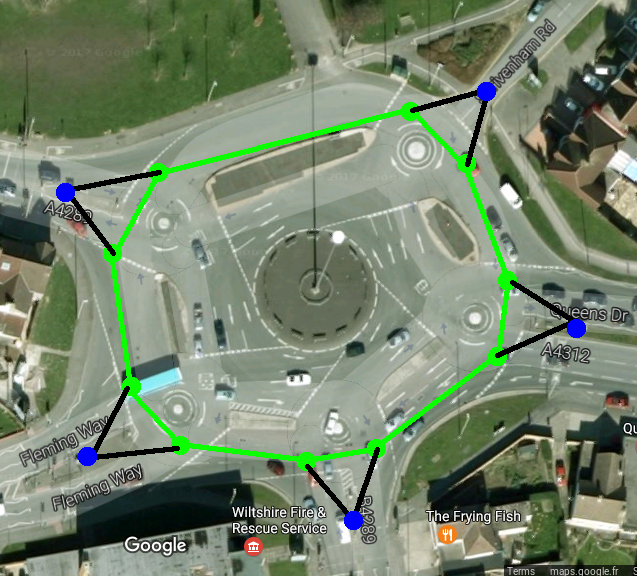
\includegraphics[scale=0.2]{../rp-graphe}}
		\end{center}	
		\caption{un graphe adapté au manège}
	\end{figure}
	
	\subsection{Réduction des distances}
Muni de ces deux graphes, on peut dès lors appliquer l'algorithme de Floyd-Warshall pour connaître la distance entre les entrées-sorties, et les comparer entre les deux graphes. Le tableau \ref{rpfw} montre le rapport des distances du manège sur celles du rond-point. Sans surprise, on remarque un gain énorme quand il s'agit de prendre la sortie située immédiatement à gauche de l'entrée, puisqu'il n'est pas nécessaire de faire tout le tour du rond-point. Le manège réduit donc bien les distances par rapport à un rond-point classique.

\begin{figure}
	\caption{\label{rpfw} Rapport entre la distance entrée-entrée pour le rond-point et le manège (en \%)}
	\begin{center}
	\begin{tabular}{ r|c c c c c}
  entrée & 0 & 4 & 8 & 12 & 16 \\ \hline
  0 & 100 & 100 & 100 & 60 & 36 \\
4 & 36 & 100 & 100 & 100 & 60 \\
8 & 60 & 36 & 100 & 100 & 100 \\
12 & 100 & 60 & 36 & 100 & 100 \\
16 & 100 & 100 & 60 & 36 & 100 \\
	\end{tabular}
	\end{center}
\end{figure}
	\subsection{Résistant aux coupures de section}
		\subsubsection{arc critique}
	Un point remarquable du manège est que, comme le montre la figure \ref{itin}, le conducteur dispose de plusieurs itinéraires pour aller d'une entrée à une sortie. Ainsi, si suite à un évènement, certaines sections se trouvent impraticables, le manège reste fonctionnel. Un algorithme permet de trouver quelles sections ne sont pas nécessaires au bon fonctionnement du manège. Défini formellement :
\begin{defin}
	Soit $G = (V,E)$ un graphe orienté. L'arc $(a,b) \in E$ est dit critique si le graphe $G^\prime = (V,E\backslash \{(a,b)\})$ n'a pas les mêmes composantes fortement connexes que $G$.
\end{defin}
Un théorème intéressant nous permet de déterminer de tels arcs : 
\begin{theo}
		Soit $G=(V,E)$ un graphe orienté fortement connexe, $(a,b) \in E$, alors :
		$G^\prime = (V,E\backslash \{ (a,b) \})$ est fortement connexe SSI il existe un chemin de $a$ à $b$
		dans $G^\prime$
\end{theo}
Pour savoir si $(a,b)$ est un arc critique, il suffit donc de déterminer si $b$ est atteignable depuis $a$ dans $G\prime$, à l'aide d'un simple parcours du graphe.
		\subsubsection{implantation et complexité}
	Considérons un graphe $G=(V,E)$. L'algorithme fonctionne donc sur le principe décrit ci-dessus : On dispose de la liste des arcs critiques, initialement vide. Pour chaque arête $(a,b)$ du graphe, on supprime cette arête (on a $G\prime$), si $b$ n'est pas accessible depuis $a$ dans $G\prime$, alors on ajoute $(a,b)$ à la liste des arcs critiques, puis on rajoute $(a,b)$ à $G\prime$.\par 
Le besoin de supprimer des arêtes pousse à choisir la structure de matrice d'adjacence (voir \ref{grmli}) pour représenter le graphe, suppression effectuée pour cette structure en temps constant. Dans ce cas, on rappelle la complexité en temps d'un parcours de $G$ : $O(|V|^2)$. \par 
Lors de l'exécution de l'algorithme, on effectue donc :
\begin{itemize}
	\item Des opérations en temps constant
	\item Un parcours des arêtes de $G$, en un temps $O(|V|^2)$
	\item $|E|$ fois :
	\begin{itemize}
		\item des opérations en temps constant (suppression, ajout…)
		\item Un parcours d'un graphe à $(|V|)$ sommets, en temps $O(|V|^2$
	\end{itemize}
\end{itemize}

La complexité totale de l'algorithme est donc un $O(|V|^2 + |E||V|^2) = O(|E||V|^2)$

\section{Un Modèle par automate cellulaire}
	\subsection{Automate cellulaire}
	\subsection{Le Problème des intersections}
	\subsection{Étude locale}
	\subsection{Limites du modèle pour le manège}
	
\section{Annexe}
	\subsection{Graphe du manège}

\label{grmli}
\verb+ graphe.mli+
\lstinputlisting{./../graphe.mli}

\verb+ graphe.ml+
\lstinputlisting{./../graphe.ml}
	\subsection{Automate cellulaire}

\end{document}